% =============================================================================
% LaTeX Full Feature Demo - 완전한 기능 데모 문서
% macOS + TeX Live 2025 + XeLaTeX/LuaLaTeX 환경용
% =============================================================================

\documentclass[a4paper, 11pt]{article}

% --- 기본 설정 ---
\usepackage[a4paper, top=2cm, bottom=2cm, left=2cm, right=2cm]{geometry}
\usepackage{fontspec}
\usepackage[bidi=default]{babel}
\babelprovide[main, import]{korean}
\babelprovide[import]{english}

% --- 한글 기본 폰트 설정 ---
\babelfont{rm}{Noto Serif CJK KR}
\babelfont{sf}{Noto Sans CJK KR}
\babelfont{tt}{Noto Sans CJK KR}

% --- 필수 패키지 ---
\usepackage{xcolor}           % 색상
\usepackage{graphicx}         % 이미지
\usepackage{tikz}             % 그래픽
\usetikzlibrary{shapes, arrows.meta, positioning, calc, decorations.pathreplacing, patterns, shadows, trees, mindmap, calendar, backgrounds}
\usepackage{pgfplots}         % 차트/그래프
\pgfplotsset{compat=1.18}
\usepackage{tcolorbox}        % 색상 박스
\tcbuselibrary{skins, breakable, listings, theorems}
\usepackage{listings}         % 코드 리스팅
\usepackage{booktabs}         % 전문적 표
\usepackage{tabularx}         % 자동 너비 표
\usepackage{longtable}        % 긴 표
\usepackage{multirow}         % 다중 행
\usepackage{multicol}         % 다중 열 레이아웃
\usepackage{enumitem}         % 목록 커스터마이징
\usepackage{amsmath, amssymb, amsthm} % 수학
\usepackage{mathtools}        % 수학 도구
\usepackage{unicode-math}     % 유니코드 수학
\usepackage{fontawesome5}     % 아이콘
\usepackage{hyperref}         % 하이퍼링크
\usepackage{fancyhdr}         % 머리말/꼬리말
\usepackage{titlesec}         % 섹션 스타일링
\usepackage{setspace}         % 줄간격
\usepackage{float}            % 그림 위치
\usepackage{wrapfig}          % 텍스트 감싸기
\usepackage{subcaption}       % 서브 캡션
\usepackage{lipsum}           % 더미 텍스트
\usepackage{qrcode}           % QR 코드
\usepackage{datetime2}        % 날짜/시간
\usepackage{pifont}           % 딩벳 기호
\usepackage{forest}           % 트리 구조
\usepackage{chemfig}          % 화학식
\usepackage{circuitikz}       % 회로도
\usepackage{pgf-pie}          % 원형 차트

% --- 색상 정의 ---
\definecolor{codegreen}{rgb}{0,0.6,0}
\definecolor{codegray}{rgb}{0.5,0.5,0.5}
\definecolor{codepurple}{rgb}{0.58,0,0.82}
\definecolor{backcolour}{rgb}{0.95,0.95,0.92}
\definecolor{myblue}{RGB}{0, 102, 204}
\definecolor{mygreen}{RGB}{0, 153, 76}
\definecolor{myred}{RGB}{204, 0, 51}
\definecolor{myyellow}{RGB}{255, 204, 0}
\definecolor{mypurple}{RGB}{128, 0, 128}

% --- 코드 스타일 ---
\lstdefinestyle{mystyle}{
    backgroundcolor=\color{backcolour},   
    commentstyle=\color{codegreen},
    keywordstyle=\color{magenta},
    numberstyle=\tiny\color{codegray},
    stringstyle=\color{codepurple},
    basicstyle=\ttfamily\footnotesize,
    breakatwhitespace=false,         
    breaklines=true,                 
    captionpos=b,                    
    keepspaces=true,                 
    numbers=left,                    
    numbersep=5pt,                  
    showspaces=false,                
    showstringspaces=false,
    showtabs=false,                  
    tabsize=2,
    frame=single,
    rulecolor=\color{black}
}
\lstset{style=mystyle}

% --- 하이퍼링크 설정 ---
\hypersetup{
    colorlinks=true,
    linkcolor=myblue,
    filecolor=magenta,      
    urlcolor=cyan,
    pdftitle={LaTeX Full Demo},
    pdfauthor={Demo Author}
}

% --- 정리 환경 설정 ---
\newtheorem{theorem}{정리}[section]
\newtheorem{lemma}[theorem]{보조정리}
\newtheorem{definition}{정의}[section]
\theoremstyle{remark}
\newtheorem*{remark}{참고}

% --- 문서 정보 ---
\title{\textbf{\Huge LaTeX 완전 기능 데모} \\[0.5em] 
       \Large Full Feature Demonstration for macOS TeX Live 2025}
\author{데모 문서 - Demo Document}
\date{\today}

\begin{document}

% =============================================================================
% 표지
% =============================================================================
\maketitle
\thispagestyle{empty}

\begin{center}
\vspace{1cm}
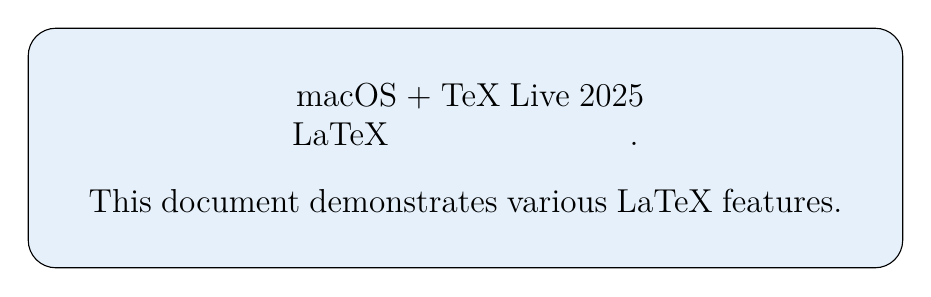
\begin{tikzpicture}
    \node[draw, rounded corners=10pt, fill=myblue!10, inner sep=20pt, text width=0.8\textwidth, align=center] {
        \large 이 문서는 macOS + TeX Live 2025 환경에서 \\
        LaTeX의 다양한 기능을 시연하기 위한 데모 문서입니다.\\[1em]
        This document demonstrates various LaTeX features.
    };
\end{tikzpicture}
\end{center}

\newpage
\tableofcontents
\newpage

% =============================================================================
% 1. 폰트 쇼케이스
% =============================================================================
\section{폰트 쇼케이스 / Font Showcase}

\subsection{한글 폰트 (Korean Fonts)}

다음은 현재 시스템에 설치된 한글 폰트들입니다:

\begin{tcolorbox}[colback=blue!5!white, colframe=blue!75!black, title={\faFont\ 한글 폰트 목록}]

% --- Noto Serif CJK KR ---
\textbf{1. Noto Serif CJK KR (노토 세리프)}

{\fontspec{Noto Serif CJK KR}
가나다라마바사 아자차카타파하 \\
동해물과 백두산이 마르고 닳도록 하느님이 보우하사 우리나라 만세}

{\fontspec{Noto Serif CJK KR Light}
\textit{Light:} 가나다라마바사 동해물과 백두산이}

{\fontspec{Noto Serif CJK KR SemiBold}
\textbf{SemiBold:} 가나다라마바사 동해물과 백두산이}

{\fontspec{Noto Serif CJK KR Black}
\textbf{Black:} 가나다라마바사 동해물과 백두산이}

\tcblower

% --- Noto Sans CJK KR ---
\textbf{2. Noto Sans CJK KR (노토 산스)}

{\fontspec{Noto Sans CJK KR}
가나다라마바사 아자차카타파하 \\
동해물과 백두산이 마르고 닳도록 하느님이 보우하사 우리나라 만세}

{\fontspec{Noto Sans CJK KR Light}
\textit{Light:} 가나다라마바사 동해물과 백두산이}

{\fontspec{Noto Sans CJK KR Medium}
\textbf{Medium:} 가나다라마바사 동해물과 백두산이}

{\fontspec{Noto Sans CJK KR Black}
\textbf{Black:} 가나다라마바사 동해물과 백두산이}

\end{tcolorbox}

\vspace{1em}

\begin{tcolorbox}[colback=green!5!white, colframe=green!75!black, title={\faFont\ 나눔 폰트 시리즈}]

% --- 나눔고딕 ---
\textbf{3. 나눔고딕 (NanumGothic)}

{\fontspec{NanumGothic}
가나다라마바사 아자차카타파하 \\
동해물과 백두산이 마르고 닳도록 하느님이 보우하사 우리나라 만세}

{\fontspec{NanumGothic ExtraBold}
\textbf{ExtraBold:} 가나다라마바사 동해물과 백두산이}

\tcblower

% --- 나눔명조 ---
\textbf{4. 나눔명조 (NanumMyeongjo)}

{\fontspec{NanumMyeongjo}
가나다라마바사 아자차카타파하 \\
동해물과 백두산이 마르고 닳도록 하느님이 보우하사 우리나라 만세}

{\fontspec{NanumMyeongjoExtraBold}
\textbf{ExtraBold:} 가나다라마바사 동해물과 백두산이}

\end{tcolorbox}

\vspace{1em}

\begin{tcolorbox}[colback=orange!5!white, colframe=orange!75!black, title={\faFont\ 나눔스퀘어 네오 \& 손글씨}]

% --- 나눔스퀘어 네오 ---
\textbf{5. 나눔스퀘어 네오 (NanumSquare Neo)}

{\fontspec{NanumSquare Neo Light}
Light: 가나다라마바사 동해물과 백두산이}

{\fontspec{NanumSquare Neo Regular}
Regular: 가나다라마바사 동해물과 백두산이}

{\fontspec{NanumSquare Neo Bold}
Bold: 가나다라마바사 동해물과 백두산이}

{\fontspec{NanumSquare Neo ExtraBold}
ExtraBold: 가나다라마바사 동해물과 백두산이}

{\fontspec{NanumSquare Neo Heavy}
Heavy: 가나다라마바사 동해물과 백두산이}

\tcblower

% --- 나눔손글씨 ---
\textbf{6. 나눔손글씨 (Nanum Brush/Pen Script)}

{\fontspec{Nanum Brush Script}
붓글씨: 가나다라마바사 동해물과 백두산이 마르고 닳도록}

{\fontspec{Nanum Pen Script}
펜글씨: 가나다라마바사 동해물과 백두산이 마르고 닳도록}

\end{tcolorbox}

\vspace{1em}

\begin{tcolorbox}[colback=purple!5!white, colframe=purple!75!black, title={\faFont\ Apple 기본 한글 폰트}]

% --- Apple SD Gothic Neo ---
\textbf{7. Apple SD 산돌고딕 Neo}

{\fontspec{Apple SD Gothic Neo}
가나다라마바사 아자차카타파하 \\
동해물과 백두산이 마르고 닳도록 하느님이 보우하사 우리나라 만세}

\tcblower

% --- AppleMyungjo ---
\textbf{8. AppleMyungjo (애플명조)}

{\fontspec{AppleMyungjo}
가나다라마바사 아자차카타파하 \\
동해물과 백두산이 마르고 닳도록 하느님이 보우하사 우리나라 만세}

\tcblower

% --- AppleGothic ---
\textbf{9. AppleGothic (애플고딕)}

{\fontspec{AppleGothic}
가나다라마바사 아자차카타파하 동해물과 백두산이}

\end{tcolorbox}

\vspace{1em}

\begin{tcolorbox}[colback=red!5!white, colframe=red!75!black, title={\faFont\ 배달의민족 폰트}]

% --- 배달의민족 폰트들 ---
\textbf{10. 배달의민족 도현 (BM Dohyeon)}

{\fontspec{BM Dohyeon OTF}
가나다라마바사 아자차카타파하 동해물과 백두산이 마르고 닳도록}

\tcblower

\textbf{11. 배달의민족 연성 (BM Yeonsung)}

{\fontspec{BM YEONSUNG OTF}
가나다라마바사 아자차카타파하 동해물과 백두산이 마르고 닳도록}

\tcblower

\textbf{12. 배달의민족 기랑해랑 (BM Kirang Haerang)}

{\fontspec{BM KIRANGHAERANG OTF}
가나다라마바사 아자차카타파하 동해물과 백두산이}

\end{tcolorbox}

\vspace{1em}

\begin{tcolorbox}[colback=gray!5!white, colframe=gray!75!black, title={\faFont\ 기타 한글 폰트}]

% --- KoPub바탕체 ---
\textbf{13. KoPub바탕체 (KoPub Batang)}

{\fontspec{KoPub Batang}
가나다라마바사 아자차카타파하 \\
동해물과 백두산이 마르고 닳도록 하느님이 보우하사 우리나라 만세}

\tcblower

% --- 전통 폰트 ---
\textbf{14. 전통 스타일 폰트들}

{\fontspec{GungSeo}
궁서: 가나다라마바사 동해물과 백두산이}

{\fontspec{HeadLineA}
HeadLineA: 가나다라마바사 동해물과 백두산이}

{\fontspec{PilGi}
필기: 가나다라마바사 동해물과 백두산이}

{\fontspec{PCMyungjo}
PC명조: 가나다라마바사 동해물과 백두산이}

\end{tcolorbox}

\newpage

\subsection{영문 폰트 (English Fonts)}

다음은 현재 시스템에 설치된 주요 영문 폰트들입니다:

\begin{tcolorbox}[colback=blue!5!white, colframe=blue!75!black, title={\faFont\ 세리프 폰트 (Serif Fonts)}]

\textbf{1. Times New Roman}

{\fontspec{Times New Roman}
The quick brown fox jumps over the lazy dog. \\
ABCDEFGHIJKLMNOPQRSTUVWXYZ abcdefghijklmnopqrstuvwxyz 0123456789}

\tcblower

\textbf{2. Georgia}

{\fontspec{Georgia}
The quick brown fox jumps over the lazy dog. \\
ABCDEFGHIJKLMNOPQRSTUVWXYZ abcdefghijklmnopqrstuvwxyz 0123456789}

\tcblower

\textbf{3. Baskerville}

{\fontspec{Baskerville}
The quick brown fox jumps over the lazy dog. \\
ABCDEFGHIJKLMNOPQRSTUVWXYZ abcdefghijklmnopqrstuvwxyz 0123456789}

\end{tcolorbox}

\vspace{1em}

\begin{tcolorbox}[colback=green!5!white, colframe=green!75!black, title={\faFont\ 산세리프 폰트 (Sans-Serif Fonts)}]

\textbf{4. Arial}

{\fontspec{Arial}
The quick brown fox jumps over the lazy dog. \\
ABCDEFGHIJKLMNOPQRSTUVWXYZ abcdefghijklmnopqrstuvwxyz 0123456789}

\tcblower

\textbf{5. Helvetica Neue}

{\fontspec{Helvetica Neue}
The quick brown fox jumps over the lazy dog. \\
ABCDEFGHIJKLMNOPQRSTUVWXYZ abcdefghijklmnopqrstuvwxyz 0123456789}

\tcblower

\textbf{6. Verdana}

{\fontspec{Verdana}
The quick brown fox jumps over the lazy dog. \\
ABCDEFGHIJKLMNOPQRSTUVWXYZ abcdefghijklmnopqrstuvwxyz 0123456789}

\tcblower

\textbf{7. Avenir}

{\fontspec{Avenir}
The quick brown fox jumps over the lazy dog. \\
ABCDEFGHIJKLMNOPQRSTUVWXYZ abcdefghijklmnopqrstuvwxyz 0123456789}

\end{tcolorbox}

\vspace{1em}

\begin{tcolorbox}[colback=orange!5!white, colframe=orange!75!black, title={\faFont\ 모노스페이스 폰트 (Monospace Fonts)}]

\textbf{8. Courier New}

{\fontspec{Courier New}
The quick brown fox jumps over the lazy dog. \\
ABCDEFGHIJKLMNOPQRSTUVWXYZ abcdefghijklmnopqrstuvwxyz 0123456789}

\tcblower

\textbf{9. Menlo}

{\fontspec{Menlo}
The quick brown fox jumps over the lazy dog. \\
ABCDEFGHIJKLMNOPQRSTUVWXYZ abcdefghijklmnopqrstuvwxyz 0123456789}

\tcblower

\textbf{10. Monaco}

{\fontspec{Monaco}
The quick brown fox jumps over the lazy dog. \\
ABCDEFGHIJKLMNOPQRSTUVWXYZ abcdefghijklmnopqrstuvwxyz 0123456789}

\end{tcolorbox}

\newpage

% =============================================================================
% 2. 수학 기능
% =============================================================================
\section{수학 기능 / Mathematics}

LaTeX의 강력한 수학 조판 기능을 시연합니다.

\subsection{기본 수식 (Basic Equations)}

인라인 수식: 아인슈타인의 질량-에너지 등가 공식 $E = mc^2$ 와 피타고라스 정리 $a^2 + b^2 = c^2$.

\begin{equation}
    \int_0^\infty e^{-x^2} dx = \frac{\sqrt{\pi}}{2}
    \label{eq:gaussian}
\end{equation}

\subsection{정렬된 수식 (Aligned Equations)}

\begin{align}
    (a+b)^2 &= a^2 + 2ab + b^2 \\
    (a-b)^2 &= a^2 - 2ab + b^2 \\
    (a+b)(a-b) &= a^2 - b^2
\end{align}

\subsection{행렬 (Matrices)}

\[
A = \begin{pmatrix}
    a_{11} & a_{12} & a_{13} \\
    a_{21} & a_{22} & a_{23} \\
    a_{31} & a_{32} & a_{33}
\end{pmatrix}, \quad
B = \begin{bmatrix}
    1 & 2 & 3 \\
    4 & 5 & 6 \\
    7 & 8 & 9
\end{bmatrix}, \quad
C = \begin{vmatrix}
    x & y \\
    z & w
\end{vmatrix}
\]

\subsection{분수 및 적분 (Fractions and Integrals)}

\begin{equation}
    \frac{d}{dx}\left[\int_a^x f(t)\,dt\right] = f(x)
\end{equation}

\begin{equation}
    \iiint_V \left(\frac{\partial P}{\partial x} + \frac{\partial Q}{\partial y} + \frac{\partial R}{\partial z}\right) dV = \oiint_S \mathbf{F} \cdot d\mathbf{S}
\end{equation}

\subsection{미분방정식 (Differential Equations)}

\begin{equation}
    \frac{\partial^2 u}{\partial t^2} = c^2 \nabla^2 u = c^2 \left(\frac{\partial^2 u}{\partial x^2} + \frac{\partial^2 u}{\partial y^2} + \frac{\partial^2 u}{\partial z^2}\right)
\end{equation}

\subsection{급수와 극한 (Series and Limits)}

\begin{equation}
    e^x = \sum_{n=0}^{\infty} \frac{x^n}{n!} = 1 + x + \frac{x^2}{2!} + \frac{x^3}{3!} + \cdots
\end{equation}

\begin{equation}
    \lim_{n \to \infty} \left(1 + \frac{1}{n}\right)^n = e \approx 2.71828\ldots
\end{equation}

\subsection{정리 환경 (Theorem Environments)}

\begin{definition}
함수 $f: \mathbb{R} \to \mathbb{R}$가 점 $a$에서 \textbf{연속}이라 함은 
\[
\lim_{x \to a} f(x) = f(a)
\]
가 성립하는 것을 말한다.
\end{definition}

\begin{theorem}[중간값 정리]
$f$가 폐구간 $[a, b]$에서 연속이고 $f(a) \neq f(b)$이면, $f(a)$와 $f(b)$ 사이의 임의의 값 $k$에 대하여 $f(c) = k$인 $c \in (a, b)$가 존재한다.
\end{theorem}

\begin{proof}
일반성을 잃지 않고 $f(a) < k < f(b)$라 가정하자. 집합 $S = \{x \in [a,b] : f(x) < k\}$는 유계이고 비어있지 않다. 
$c = \sup S$라 하면, 연속성에 의해 $f(c) = k$임을 보일 수 있다.
\end{proof}

\begin{remark}
이 정리는 연속함수의 본질적인 성질을 나타냅니다.
\end{remark}

\newpage

% =============================================================================
% 3. 표 / Tables
% =============================================================================
\section{표 / Tables}

\subsection{기본 표}

\begin{table}[H]
\centering
\caption{기본 표 예제}
\begin{tabular}{|l|c|r|}
\hline
\textbf{항목} & \textbf{수량} & \textbf{가격} \\
\hline
사과 & 10개 & 5,000원 \\
바나나 & 5묶음 & 7,500원 \\
오렌지 & 8개 & 6,400원 \\
\hline
\textbf{합계} & & \textbf{18,900원} \\
\hline
\end{tabular}
\end{table}

\subsection{전문적인 표 (Booktabs)}

\begin{table}[H]
\centering
\caption{booktabs 패키지를 사용한 전문적인 표}
\begin{tabular}{@{}lrrr@{}}
\toprule
\textbf{과목명} & \textbf{학점} & \textbf{점수} & \textbf{등급} \\
\midrule
미적분학 & 3 & 95 & A+ \\
선형대수학 & 3 & 88 & B+ \\
확률과 통계 & 3 & 92 & A \\
이산수학 & 3 & 85 & B \\
\midrule
\textbf{평균} & \textbf{12} & \textbf{90} & \textbf{A} \\
\bottomrule
\end{tabular}
\end{table}

\subsection{다중 행/열 표}

\begin{table}[H]
\centering
\caption{다중 행과 열이 있는 복잡한 표}
\begin{tabular}{|c|c|c|c|c|}
\hline
\multirow{2}{*}{\textbf{학년}} & \multicolumn{2}{c|}{\textbf{1학기}} & \multicolumn{2}{c|}{\textbf{2학기}} \\
\cline{2-5}
 & 중간 & 기말 & 중간 & 기말 \\
\hline
1학년 & 85 & 88 & 90 & 92 \\
2학년 & 78 & 82 & 85 & 88 \\
3학년 & 92 & 95 & 93 & 97 \\
\hline
\end{tabular}
\end{table}

\subsection{색상이 있는 표}

\begin{table}[H]
\centering
\caption{색상이 적용된 표}
\begin{tabular}{|>{\columncolor{myblue!20}}l|c|c|c|}
\hline
\rowcolor{myblue!40}
\textbf{분류} & \textbf{항목 A} & \textbf{항목 B} & \textbf{항목 C} \\
\hline
카테고리 1 & \cellcolor{mygreen!20}높음 & 중간 & 낮음 \\
카테고리 2 & 낮음 & \cellcolor{myyellow!30}중간 & 높음 \\
카테고리 3 & 중간 & 높음 & \cellcolor{myred!20}낮음 \\
\hline
\end{tabular}
\end{table}

\newpage

% =============================================================================
% 4. 그래픽 / Graphics
% =============================================================================
\section{그래픽 / Graphics (TikZ)}

\subsection{기본 도형}

\begin{center}

\begin{tikzpicture}
    % 사각형
    \draw[fill=myblue!30] (0,0) rectangle (2,1.5);
    \node at (1, 0.75) {사각형};
    
    % 원
    \draw[fill=mygreen!30] (4,0.75) circle (0.75);
    \node at (4, 0.75) {원};
    
    % 타원
    \draw[fill=myyellow!30] (7,0.75) ellipse (1 and 0.5);
    \node at (7, 0.75) {타원};
    
    % 삼각형
    \draw[fill=myred!30] (10,0) -- (11.5,0) -- (10.75,1.5) -- cycle;
    \node at (10.75, 0.5) {삼각형};
\end{tikzpicture}
\end{center}

\subsection{화살표와 선}

\begin{center}
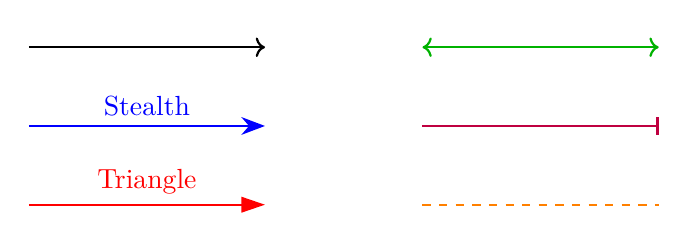
\begin{tikzpicture}
    % 다양한 화살표 스타일
    \draw[->, thick] (0,2) -- (3,2) node[midway, above] {일반 화살표};
    \draw[-{Stealth[length=3mm]}, thick, blue] (0,1) -- (3,1) node[midway, above] {Stealth};
    \draw[-{Triangle[length=3mm]}, thick, red] (0,0) -- (3,0) node[midway, above] {Triangle};
    \draw[<->, thick, green!70!black] (5,2) -- (8,2) node[midway, above] {양방향};
    \draw[-|, thick, purple] (5,1) -- (8,1) node[midway, above] {막대 끝};
    \draw[dashed, thick, orange] (5,0) -- (8,0) node[midway, above] {점선};
\end{tikzpicture}
\end{center}

\subsection{플로우차트}

\begin{center}
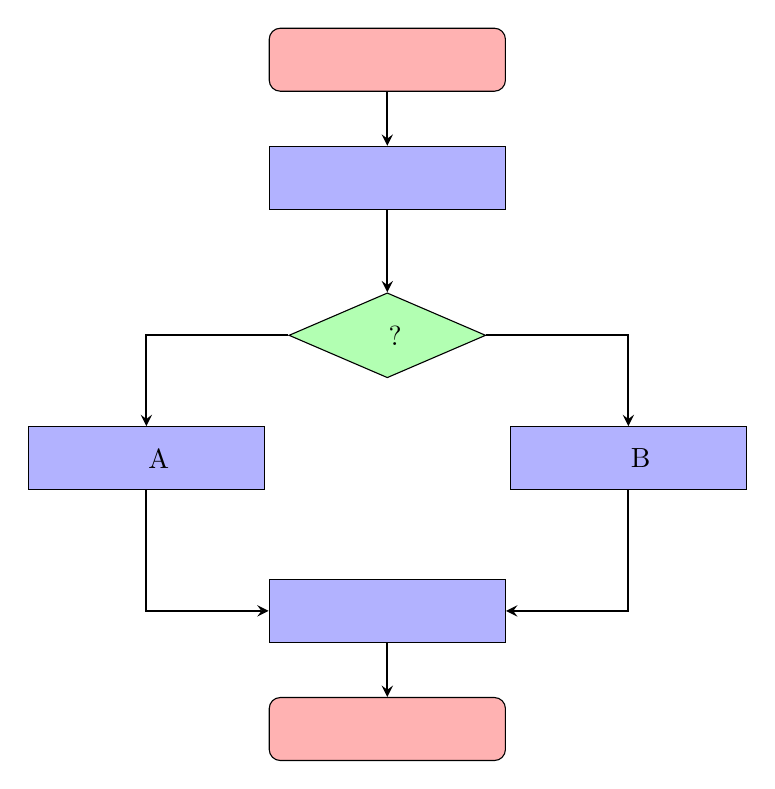
\begin{tikzpicture}[node distance=1.5cm,
    startstop/.style={rectangle, rounded corners, minimum width=3cm, minimum height=0.8cm, text centered, draw=black, fill=red!30},
    process/.style={rectangle, minimum width=3cm, minimum height=0.8cm, text centered, draw=black, fill=blue!30},
    decision/.style={diamond, minimum width=2.5cm, minimum height=1cm, text centered, draw=black, fill=green!30},
    arrow/.style={thick,->,>=stealth}]

    \node (start) [startstop] {시작};
    \node (input) [process, below of=start] {입력 받기};
    \node (decide) [decision, below of=input, yshift=-0.5cm] {조건?};
    \node (process1) [process, below left of=decide, xshift=-2cm, yshift=-0.5cm] {처리 A};
    \node (process2) [process, below right of=decide, xshift=2cm, yshift=-0.5cm] {처리 B};
    \node (output) [process, below of=decide, yshift=-2cm] {출력};
    \node (stop) [startstop, below of=output] {종료};

    \draw [arrow] (start) -- (input);
    \draw [arrow] (input) -- (decide);
    \draw [arrow] (decide) -| node[near start, above] {예} (process1);
    \draw [arrow] (decide) -| node[near start, above] {아니오} (process2);
    \draw [arrow] (process1) |- (output);
    \draw [arrow] (process2) |- (output);
    \draw [arrow] (output) -- (stop);
\end{tikzpicture}
\end{center}

\subsection{마인드맵}

\begin{center}
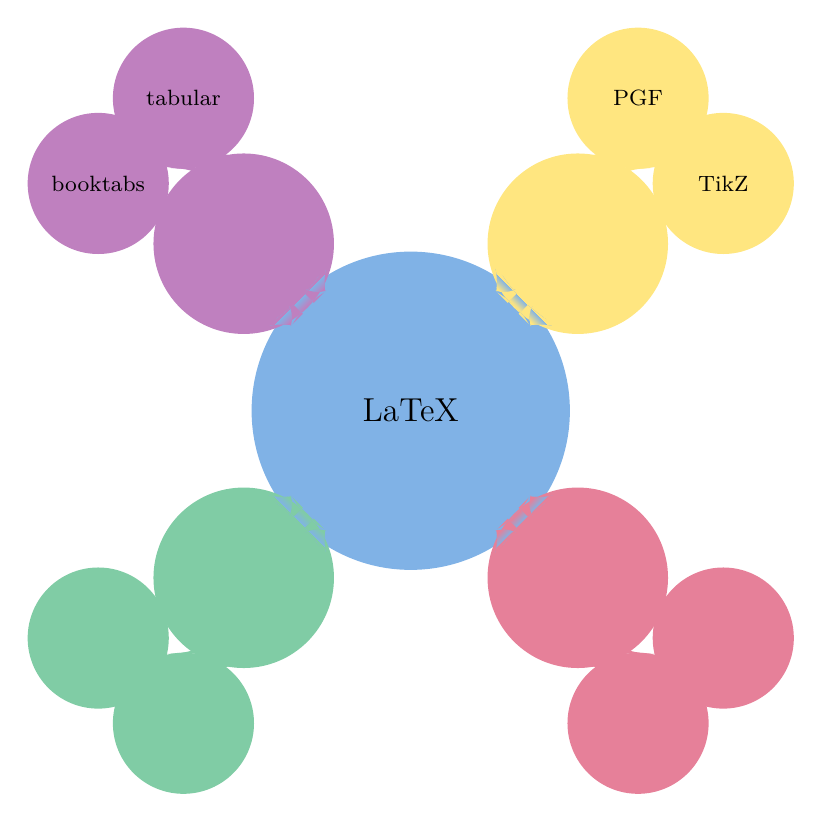
\begin{tikzpicture}[mindmap, grow cyclic, every node/.style={concept},
    concept color=myblue!50,
    level 1/.append style={level distance=3cm, sibling angle=90},
    level 2/.append style={level distance=2cm, sibling angle=45}]
    
    \node {LaTeX}
        child[concept color=mygreen!50] { node {문서 작성}
            child { node {논문} }
            child { node {보고서} }
        }
        child[concept color=myred!50] { node {수식}
            child { node {방정식} }
            child { node {행렬} }
        }
        child[concept color=myyellow!50] { node {그래픽}
            child { node {TikZ} }
            child { node {PGF} }
        }
        child[concept color=mypurple!50] { node {표}
            child { node {tabular} }
            child { node {booktabs} }
        };
\end{tikzpicture}
\end{center}

\newpage

\subsection{그래프 (PGFPlots)}

\begin{center}
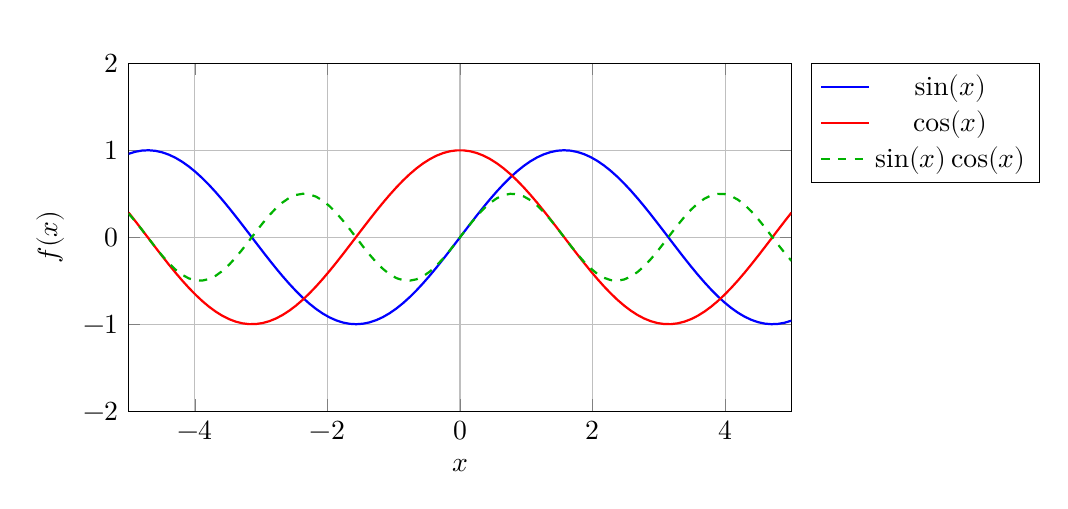
\begin{tikzpicture}
\begin{axis}[
    width=10cm, height=6cm,
    xlabel={$x$},
    ylabel={$f(x)$},
    title={다양한 함수 그래프},
    legend pos=outer north east,
    grid=major,
    xmin=-5, xmax=5,
    ymin=-2, ymax=2
]
    \addplot[blue, thick, domain=-5:5, samples=100] {sin(deg(x))};
    \addlegendentry{$\sin(x)$}
    
    \addplot[red, thick, domain=-5:5, samples=100] {cos(deg(x))};
    \addlegendentry{$\cos(x)$}
    
    \addplot[green!70!black, thick, dashed, domain=-5:5, samples=100] {sin(deg(x))*cos(deg(x))};
    \addlegendentry{$\sin(x)\cos(x)$}
\end{axis}
\end{tikzpicture}
\end{center}

\vspace{1em}

\begin{center}
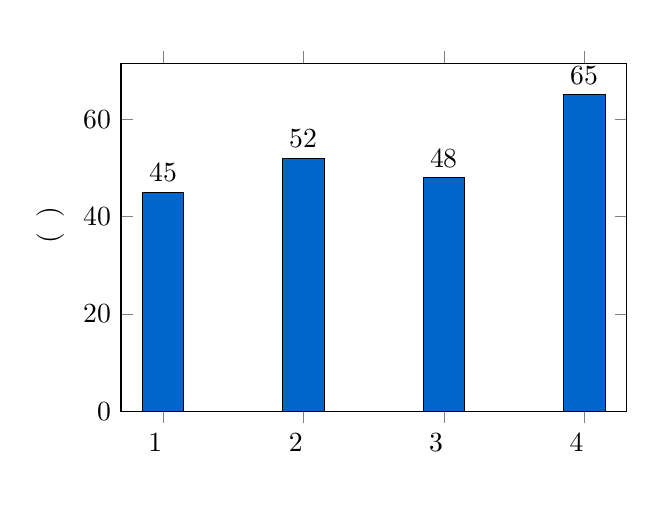
\begin{tikzpicture}
\begin{axis}[
    width=8cm, height=6cm,
    ybar,
    xlabel={분기},
    ylabel={매출 (억원)},
    title={분기별 매출 현황},
    symbolic x coords={1분기, 2분기, 3분기, 4분기},
    xtick=data,
    nodes near coords,
    bar width=15pt,
    ymin=0
]
    \addplot[fill=myblue] coordinates {(1분기,45) (2분기,52) (3분기,48) (4분기,65)};
\end{axis}
\end{tikzpicture}
\end{center}

\begin{center}
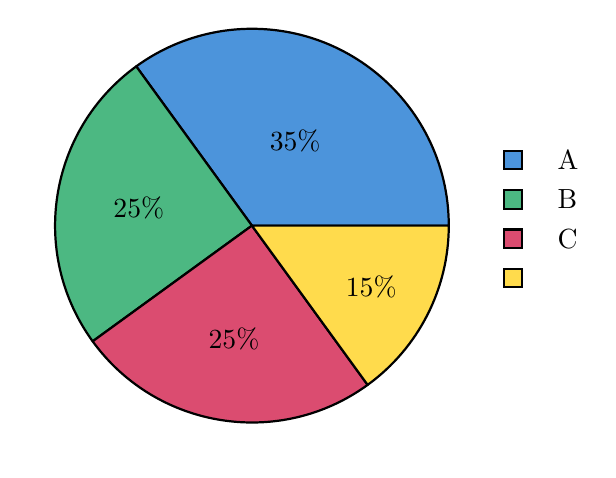
\begin{tikzpicture}
  \pie[text=legend, radius=2.5, color={myblue!70, mygreen!70, myred!70, myyellow!70}]{
    35/제품 A,
    25/제품 B,
    25/제품 C,
    15/기타
  }
\end{tikzpicture}
\end{center}

\newpage

% =============================================================================
% 5. 코드 리스팅
% =============================================================================
\section{코드 리스팅 / Code Listings}

\subsection{Python 코드}

\begin{lstlisting}[language=Python, caption={Python 예제 - Hello World와 함수}]
#!/usr/bin/env python3
# -*- coding: utf-8 -*-
"""
LaTeX Demo - Python Code Example
"""

def greet(name: str) -> str:
    """인사말을 반환하는 함수"""
    return f"안녕하세요, {name}님!"

class Calculator:
    """간단한 계산기 클래스"""
    
    def add(self, a: float, b: float) -> float:
        return a + b
    
    def subtract(self, a: float, b: float) -> float:
        return a - b

if __name__ == "__main__":
    print(greet("LaTeX"))
    calc = Calculator()
    print(f"5 + 3 = {calc.add(5, 3)}")
\end{lstlisting}

\subsection{JavaScript 코드}

\begin{lstlisting}[language=JavaScript, caption={JavaScript 예제}]
// LaTeX Demo - JavaScript Example
const greeting = (name) => {
    return `Hello, ${name}!`;
};

class Rectangle {
    constructor(width, height) {
        this.width = width;
        this.height = height;
    }
    
    get area() {
        return this.width * this.height;
    }
}

console.log(greeting("World"));
const rect = new Rectangle(10, 5);
console.log(`Area: ${rect.area}`);
\end{lstlisting}

\subsection{LaTeX 코드}

\begin{lstlisting}[language={[LaTeX]TeX}, caption={LaTeX 예제}]
\documentclass{article}
\usepackage{amsmath}

\begin{document}
    \title{My Document}
    \author{Author Name}
    \maketitle
    
    \section{Introduction}
    This is a sample document.
    
    \begin{equation}
        E = mc^2
    \end{equation}
\end{document}
\end{lstlisting}

\newpage

% =============================================================================
% 6. 박스와 프레임
% =============================================================================
\section{박스와 프레임 / Boxes \& Frames}

\subsection{tcolorbox 스타일}

\begin{tcolorbox}[colback=blue!5!white, colframe=blue!75!black, title=정보 박스]
\faInfoCircle\ 이것은 정보를 표시하는 박스입니다. 중요한 내용을 강조할 때 사용합니다.
\end{tcolorbox}

\begin{tcolorbox}[colback=green!5!white, colframe=green!75!black, title=\faCheckCircle\ 성공]
작업이 성공적으로 완료되었습니다!
\end{tcolorbox}

\begin{tcolorbox}[colback=yellow!10!white, colframe=yellow!75!black, title=\faExclamationTriangle\ 경고]
주의가 필요한 내용입니다. 신중하게 진행하세요.
\end{tcolorbox}

\begin{tcolorbox}[colback=red!5!white, colframe=red!75!black, title=\faTimesCircle\ 오류]
오류가 발생했습니다. 설정을 확인해 주세요.
\end{tcolorbox}

\subsection{그림자 효과}

\begin{tcolorbox}[enhanced, drop shadow southeast, colback=white, colframe=gray]
이 박스에는 그림자 효과가 적용되어 있습니다.
\end{tcolorbox}

\subsection{분할 박스}

\begin{tcolorbox}[colback=blue!5!white, colframe=blue!75!black, title=분할 박스, sidebyside]
\textbf{왼쪽 영역}

이곳에 왼쪽 내용을 작성합니다.
\tcblower
\textbf{오른쪽 영역}

이곳에 오른쪽 내용을 작성합니다.
\end{tcolorbox}

\newpage

% =============================================================================
% 7. 목록과 열거
% =============================================================================
\section{목록과 열거 / Lists \& Enumerations}

\subsection{기본 목록}

\begin{multicols}{2}
\textbf{순서 없는 목록:}
\begin{itemize}
    \item 첫 번째 항목
    \item 두 번째 항목
    \begin{itemize}
        \item 중첩된 항목 A
        \item 중첩된 항목 B
    \end{itemize}
    \item 세 번째 항목
\end{itemize}

\columnbreak

\textbf{순서 있는 목록:}
\begin{enumerate}
    \item 첫 번째 단계
    \item 두 번째 단계
    \begin{enumerate}
        \item 세부 단계 A
        \item 세부 단계 B
    \end{enumerate}
    \item 세 번째 단계
\end{enumerate}
\end{multicols}

\subsection{커스텀 목록 기호}

\begin{multicols}{3}
\textbf{체크 목록:}
\begin{itemize}[label=\ding{51}]
    \item 완료된 작업
    \item 완료된 작업
\end{itemize}
\begin{itemize}[label=\ding{55}]
    \item 미완료 작업
    \item 미완료 작업
\end{itemize}

\columnbreak

\textbf{화살표 목록:}
\begin{itemize}[label=\faArrowRight]
    \item 항목 A
    \item 항목 B
    \item 항목 C
\end{itemize}

\columnbreak

\textbf{별표 목록:}
\begin{itemize}[label=\faStar]
    \item 중요 항목
    \item 중요 항목
    \item 중요 항목
\end{itemize}
\end{multicols}

\subsection{설명 목록}

\begin{description}
    \item[LaTeX] 문서 조판 시스템으로, 특히 수학적 표현이 많은 문서에 적합합니다.
    \item[TikZ] LaTeX에서 복잡한 그래픽을 그릴 수 있는 패키지입니다.
    \item[BibTeX] 참고문헌 관리를 위한 도구입니다.
\end{description}

\newpage

% =============================================================================
% 8. 아이콘 (FontAwesome5)
% =============================================================================
\section{아이콘 / Icons (FontAwesome5)}

FontAwesome5 패키지를 사용한 다양한 아이콘들:

\begin{center}
\begin{tabular}{cccccc}
\faHome\ 홈 & \faUser\ 사용자 & \faCog\ 설정 & \faEnvelope\ 이메일 & \faPhone\ 전화 & \faSearch\ 검색 \\[1em]
\faGithub\ GitHub & \faTwitter\ Twitter & \faFacebook\ Facebook & \faLinkedin\ LinkedIn & \faYoutube\ YouTube & \faInstagram\ Instagram \\[1em]
\faFile\ 파일 & \faFolder\ 폴더 & \faEdit\ 편집 & \faTrash\ 삭제 & \faSave\ 저장 & \faPrint\ 인쇄 \\[1em]
\faHeart\ 좋아요 & \faStar\ 별점 & \faComment\ 댓글 & \faShare\ 공유 & \faBookmark\ 북마크 & \faBell\ 알림 \\[1em]
\faLaptop\ 노트북 & \faMobile\ 모바일 & \faDesktop\ 데스크탑 & \faTablet\ 태블릿 & \faServer\ 서버 & \faCloud\ 클라우드 \\
\end{tabular}
\end{center}

\vspace{1em}

\begin{tcolorbox}[colback=gray!5, colframe=gray!50]
\textbf{아이콘 활용 예시:}
\begin{itemize}
    \item \faCheckCircle[regular]\ 작업 완료
    \item \faTimesCircle[regular]\ 작업 취소
    \item \faExclamationTriangle\ 주의 필요
    \item \faInfoCircle\ 추가 정보
    \item \faQuestionCircle\ 도움말
\end{itemize}
\end{tcolorbox}

\newpage

% =============================================================================
% 9. QR 코드
% =============================================================================
\section{QR 코드 / QR Codes}

\begin{center}
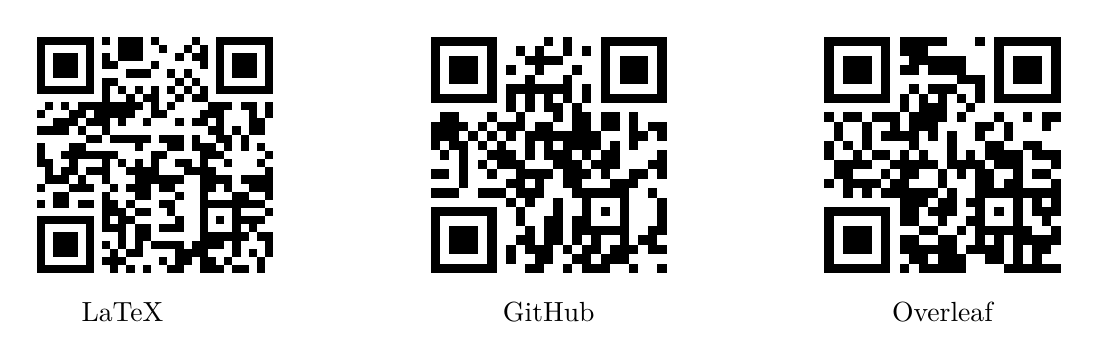
\begin{tikzpicture}
    \node at (0, 0) {\qrcode[height=3cm]{https://www.latex-project.org}};
    \node at (0, -2) {LaTeX 공식 웹사이트};
    
    \node at (5, 0) {\qrcode[height=3cm]{https://github.com}};
    \node at (5, -2) {GitHub};
    
    \node at (10, 0) {\qrcode[height=3cm]{https://www.overleaf.com}};
    \node at (10, -2) {Overleaf};
\end{tikzpicture}
\end{center}

\newpage

% =============================================================================
% 10. 특수 다이어그램
% =============================================================================
\section{특수 다이어그램 / Special Diagrams}

\subsection{트리 구조 (Forest)}

\begin{center}
\begin{forest}
for tree={
    grow'=0,
    child anchor=west,
    parent anchor=east,
    anchor=west,
    l sep=10mm,
    edge path={
        \noexpand\path [draw, \forestoption{edge}] (!u.parent anchor) -- +(5pt,0) |- (.child anchor)\forestoption{edge label};
    }
}
[프로젝트 구조
    [src
        [main.py]
        [utils.py]
        [config.py]
    ]
    [docs
        [README.md]
        [API.md]
    ]
    [tests
        [test\_main.py]
        [test\_utils.py]
    ]
]
\end{forest}
\end{center}

\subsection{화학식 (ChemFig)}

\begin{center}
\textbf{물 (H$_2$O):}
\quad
\chemfig{H-O-H}
\qquad\qquad
\textbf{에탄올 (C$_2$H$_5$OH):}
\quad
\chemfig{H_3C-CH_2-OH}
\end{center}

\vspace{1em}

\begin{center}
\textbf{벤젠 고리:}
\quad
\chemfig{*6(-=-=-=)}
\qquad\qquad
\textbf{카페인:}
\quad
\chemfig{
    H_3C-N*5(-C(=O)-(*6(-N=-N(-CH_3)-=))-N(-CH_3)-C(=O)-)
}
\end{center}

\subsection{전기 회로 (CircuiTikZ)}

\begin{center}
\begin{circuitikz}[american voltages]
\draw
    (0,0) to[V, l=$V_s$] (0,3)
    to[R, l=$R_1$] (3,3)
    to[R, l=$R_2$] (3,0)
    to[C, l=$C$] (0,0);
\draw
    (3,3) to[L, l=$L$] (6,3)
    to[R, l=$R_3$] (6,0)
    -- (3,0);
\end{circuitikz}
\end{center}

\newpage

% =============================================================================
% 11. 달력
% =============================================================================
\section{달력 / Calendar}

\begin{center}
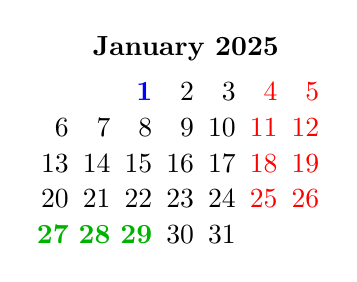
\begin{tikzpicture}
\calendar[dates=2025-01-01 to 2025-01-last,
          week list,
          month label above centered,
          month text=\textbf{\%mt \%y0}]
    if (Saturday) [red]
    if (Sunday) [red]
    if (equals=2025-01-01) [blue, font=\bfseries]
    if (between=2025-01-27 and 2025-01-29) [green!70!black, font=\bfseries];
\end{tikzpicture}
\end{center}

\newpage

% =============================================================================
% 12. 참조 및 하이퍼링크
% =============================================================================
\section{참조 및 하이퍼링크 / References \& Hyperlinks}

\subsection{내부 참조}

수식 (\ref{eq:gaussian})은 가우시안 적분을 보여줍니다.

\subsection{외부 링크}

\begin{itemize}
    \item \href{https://www.latex-project.org}{LaTeX 공식 웹사이트}
    \item \href{https://www.overleaf.com}{Overleaf - 온라인 LaTeX 편집기}
    \item \href{https://tex.stackexchange.com}{TeX Stack Exchange - Q\&A 사이트}
    \item \href{https://ctan.org}{CTAN - Comprehensive TeX Archive Network}
\end{itemize}

\subsection{이메일 링크}

문의사항은 \href{mailto:demo@example.com}{demo@example.com}으로 보내주세요.

\newpage

% =============================================================================
% 13. 색상 팔레트
% =============================================================================
\section{색상 팔레트 / Color Palette}

\subsection{기본 색상}

\begin{center}

\begin{tikzpicture}
\foreach \color [count=\i] in {red, orange, yellow, green, cyan, blue, purple, magenta, pink, brown, gray, black} {
    \fill[\color] ({mod(\i-1,6)*2}, {-floor((\i-1)/6)*1.2}) rectangle ++(1.8, 1);
    \node[white, font=\small\bfseries] at ({mod(\i-1,6)*2+0.9}, {-floor((\i-1)/6)*1.2+0.5}) {\color};
}
\end{tikzpicture}
\end{center}

\subsection{밝기 변형}

\begin{center}

\begin{tikzpicture}
\foreach \pct [count=\i] in {10, 25, 50, 75, 100} {
    \fill[blue!\pct] ({(\i-1)*2.2}, 0) rectangle ++(2, 1);
    \node[white, font=\small] at ({(\i-1)*2.2+1}, 0.5) {blue!\pct};
}
\end{tikzpicture}
\end{center}

\subsection{혼합 색상}

\begin{center}

\begin{tikzpicture}
\fill[red!50!blue] (0,0) rectangle (2,1);
\node[white] at (1, 0.5) {red!50!blue};

\fill[green!50!yellow] (2.5,0) rectangle (4.5,1);
\node at (3.5, 0.5) {green!50!yellow};

\fill[orange!50!black] (5,0) rectangle (7,1);
\node[white] at (6, 0.5) {orange!50!black};

\fill[cyan!50!white] (7.5,0) rectangle (9.5,1);
\node at (8.5, 0.5) {cyan!50!white};
\end{tikzpicture}
\end{center}

\newpage

% =============================================================================
% 14. 폰트 크기 비교
% =============================================================================
\section{폰트 크기 비교 / Font Size Comparison}

\begin{center}
\begin{tabular}{ll}
\toprule
\textbf{명령어} & \textbf{결과} \\
\midrule
\verb|\tiny| & {\tiny 아주 작은 텍스트 / Tiny text} \\
\verb|\scriptsize| & {\scriptsize 스크립트 크기 / Script size} \\
\verb|\footnotesize| & {\footnotesize 각주 크기 / Footnote size} \\
\verb|\small| & {\small 작은 텍스트 / Small text} \\
\verb|\normalsize| & {\normalsize 기본 크기 / Normal size} \\
\verb|\large| & {\large 큰 텍스트 / Large text} \\
\verb|\Large| & {\Large 더 큰 텍스트 / Larger text} \\
\verb|\LARGE| & {\LARGE 매우 큰 텍스트 / Even larger} \\
\verb|\huge| & {\huge 거대한 텍스트 / Huge text} \\
\verb|\Huge| & {\Huge 가장 큰 텍스트 / Largest text} \\
\bottomrule
\end{tabular}
\end{center}

% =============================================================================
% 15. 문서 끝
% =============================================================================
\section{마무리 / Conclusion}

이 문서는 LaTeX의 다양한 기능을 시연했습니다:

\begin{multicols}{2}
\begin{itemize}
    \item \faFont\ 한글/영문 폰트 쇼케이스
    \item \faCalculator\ 수학 수식
    \item \faTable\ 다양한 표
    \item \faPaintBrush\ TikZ 그래픽
    \item \faChartBar\ PGFPlots 차트
    \item \faCode\ 코드 리스팅
    \item \faSquare\ 박스와 프레임
    \item \faList\ 목록과 열거
    \item \faIcons\ FontAwesome 아이콘
    \item \faQrcode\ QR 코드
    \item \faSitemap\ 트리 구조
    \item \faFlask\ 화학식
    \item \faBolt\ 회로도
    \item \faCalendar\ 달력
    \item \faLink\ 하이퍼링크
    \item \faPalette\ 색상 팔레트
\end{itemize}
\end{multicols}

\begin{center}
\begin{tcolorbox}[colback=myblue!10, colframe=myblue, width=0.8\textwidth]
\centering
\Large\bfseries
문서 생성 완료! \\[0.5em]
\normalsize
생성일: \today \\
빌드 엔진: XeLaTeX / LuaLaTeX
\end{tcolorbox}
\end{center}

\end{document}
